\documentclass{llncs}
\usepackage{subcaption}
\usepackage{subfig} 
\usepackage{usual}
\usepackage[utf8]{inputenc}

\usepackage{graphicx}
\usepackage[rflt]{floatflt}
\usepackage[noend]{algpseudocode}
\usepackage{subfig} 
\usepackage{frame, caption}
\usepackage{amsmath}
\usepackage{eulervm}
\usepackage{fontenc}
\usepackage{mathrsfs}
\usepackage{multirow, enumitem, longtable, rotating,lipsum, scrextend}
\usepackage{array}
\usepackage{makecell}
\usepackage{xcolor, soul}
\sethlcolor{yellow}	
\usepackage{floatrow}
\newcommand{\argmax}{\operatornamewithlimits{arg\,max}}
%\pagestyle{plain}
%
\begin{document}
	\begin{abstract}
		
	\end{abstract}
%	plan of the paper
%	1. We defined a model of dialogue make a schema that explains 
%	The model produces an utterance based on the agent mental state
%	the agent mental state includes : its preferences, its representation of power noted\emph{pow}, and the context of the dialogue(history of the dialogue)
%	
%	Previous studies validated our hypotheses that the choice of the utterance as built reflect the right behaviors of power.
%	Our goal is to produce plausible social behaviors when building a relation of dominance with a human interlocutor. 
%	(Reprendre la definition de dom comme ecrite) 
%	
%	We make the assumption that our model faithfully reproduce behaviors of power when selecting utterances to enunciate. On that assumption, we aim to build a model of ToM based on simulation, able to compute the current value of power \emph{pow} expressed by the interlocutor based on the utterance expressed. 
	
	\section{Model of dialogue}
		
		We defined a dialogue system of cooperative negotiation which enable  a conversational agent to create and adapt its negotiation strategy to the power it intends to express. The goal of a negotiation is to choose an option from the discussed topic. Theses options are defined as a set of criteria  $\{C_1, ..., C_n\}$ that reflect the option's characteristics. In order to be able to negotiate about which option to choose, an agent is initiated with a set of partial or total ordered preferences $\prec_i$ defined for each criterion $C_i$. Using theses preferences, an agent can compute a score of satisfaction for each value of each criterion. The satisfaction of a value $v \in C_i$ is computed as the number of values that the agent prefers less in the preferences order $\prec_i$, then, the score is normalized in $[0, 1]$: 
		
				\begin{equation}
				sat(v, \prec_i) =	1 - \left( \frac{|\{v' : v' \neq v \  \wedge \ (v \prec_i v')\}| }{( |C_i| - 1 )}\right)
				\end{equation}
				
		The notion of satisfaction represents the score of liking for the value. The closer the satisfaction of a value $v$ gets to 1, the more the agent likes $v$. 
		
		 \subsection{Model of decision based on power}
		The decisional process during the negotiation is built to take into account the power of the agent. Therefore, agent is initiated with a value of power $pow \in [0,1]$. In addition, the decisional process to produce an utterance considers respectively, the agent's power, its preferences and the context of the negotiation.  
		
		A detailed explanation of the decisional model is presented in \cite{} . We present in the following the most important factors that defines the agent strategy.
		
		\subsubsection{Satisfiability }
		\label{sec:sat}
		The agent is allowed to share its preferences. %(\emph{StatePreference(v)}). 
		To this end, the agent considers its perception of power $pow$ to compute the satisfiability, such that a value $v$ is satisfiable (likable), if:  
		\begin{equation}
		 	sat(v, \prec_i) \geq pow
		\end{equation}
	
		Therefore, given a value of $pow$, and a model of preferences $\prec$, the agent has a set of satisfiable values noted $S$. 
		
		\par For example, consider a mental state where $pow =0.6$, a criterion with a domain $D =\{A, B, C, D\}$ is defined with the set of preferences $ \prec_D = \{A \rightarrow  B, C \rightarrow  D , B \rightarrow D \}$. The values of satisfiability are depicted in the table \ref{sat}. We can compute that the set of satisfiable values is $ S = \{B, C, D\}$ 
			 \begin{table}
			 	\centering
			 	\begin{tabular}{ |c|c|c|c|c| }
			 		\hline				
			 		value & A & B & C & D \\
			 		\hline

			 		\hline
			 		Sat(value) & 0.3 & 0.6 & 0.6 & 1 \\
			 		\hline
			 		
			 	\end{tabular}
			 	\caption{Value of satisfiability for the model $D$.}
			 	\label{sat}
			 \end{table}
		
		
	\subsubsection{Acceptability}
	 
	 During the negotiation, the agent makes decisions about the proposals it receives. It might express an \emph{Accept} or \emph{Reject}. However, when the negotiation is not converging, the agent has to make concessions which means that the agent has to lower his level of demand. 
	 We compute the notion of concession with $self(t)$, which is a time varying value of $pow$ that decreases over time $t$. In the beginning, $self(0) = pow$, when the negotiation evolves without converging self decreases $self(t) < pow$ as presented in the figure \ref{fig:conc}.
	 	\begin{floatingfigure}[r]{1.8in}
	 		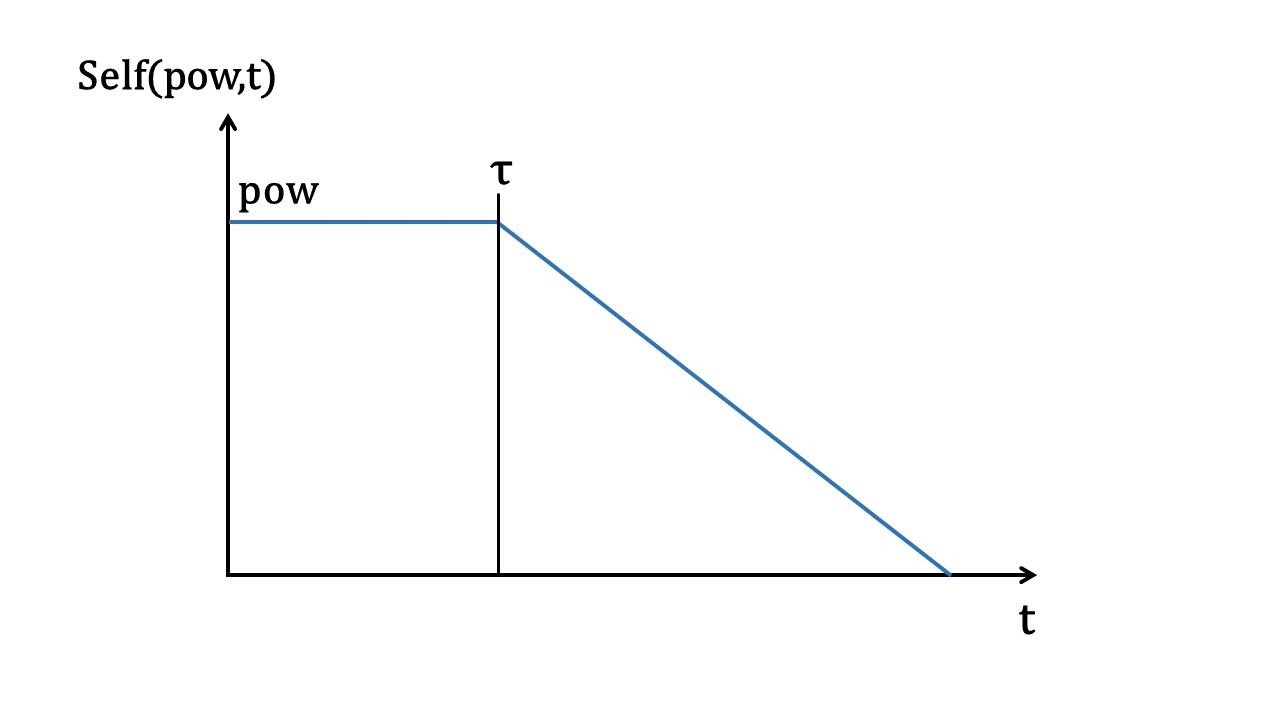
\includegraphics[width=1.8in]{figs/sv3.png}
	 		\caption{\label{fig:conc}Concession curve}
	 	\end{floatingfigure} 
	 
	Thus, a proposal with a value $v \in C_i$ is \emph{acceptable} ($v \in Ac$) is computed with a boolean function:
			\begin{equation}
				acc(pow, v) = sat(v, \prec_i) \geq self(t)
			\end{equation}	
	and we note $Ac$ the set of acceptable values.

	%When negotiation progress in time without converging to a trade-off,
	In addition, When concessions occurs during the negotiation $self(t) < pow$. As a consequence, the agent might accept proposals which are not satisfiables. We note $M$ the set of acceptable values which are not satisfiables.
	$\{v \in M / v \in Ac, v \notin S\}$.
	
%	Therefore, in order to accept \emph{Accept} or propose \emph{Propose} a value $v$, this value has to be acceptable $v \in Acc$. In the contrary, a value $v$ can be rejected (\emph{Reject}) if $v \not \in Acc$ and by consequences $v\not \in S$
%	
\subsubsection{Lead of the dialogue}
	The agent uses a strategy to choose the utterance type that reflects behaviors of power. Indeed, high-power agents focus on utterances of \emph{propose} in order to make the negotiation go on. On the contrary, a low-power agent uses in average more \emph{ask} utterances in order to have an accurate knowledge about the other to take the fairest decision.
	
	\subsection{Beliefs about other}
	
	In order to build a complementary relation of dominance with the user, the agent has to construct beliefs about the behaviors of power expressed by the user and adapt to complement his behavior. 
	
	We make the assumption that our model of dialogue effectively presents the process of utterance's selection using power. 
	
	Based on this assumption, we propose to enable the agent with a model of theory of mind based on simulation \cite{bibid}. The agent uses its model of decision in order to guess the behavior of the user from its enunciated utterance.   
	
	The agent needs to infer hypotheses about the user's mental state (\emph{i.e} Pow, Preferences) in order to reason about his behaviors. With knowledge gathered during the negotiation, the agent will remove inconsistent hypotheses.
	
	First, we define hypotheses about the possible values of $pow$ that the agents aims to predict. Let $H_{pow} = \{0.1, 0.2, \ldots, 0.9\}$ be the hypotheses on $pow$.
	
	Second, for each fixed hypothesis $ h_i \in H_{pow}$, we define hypotheses on the different set of preferences  noted $M_H $. Thus, for each criterion $C_i$ of the a topic , we compute all the possible combination of preference's relations. When relations of preferences are total ordered, the total number of preference's relations is in the order of $|H{C_i}| = |C_i|!$. In the case of partial ordered relations of preferences, the total number of possible relations is  $ |H{C_i}| = (|C_i| + 1)!$. Hence, for a topic of negotiation with $n$ criteria, the number of possible set of preferences is $$ |M_H| = \prod_{i=1}^n (|H{C_i}|)$$. 
	
	For each hypothesis $ h_i \in H_{pow}$, we associate the set of possible preferences $M_H(h_i)$ identical for all the hypotheses in the beginning. After each user's turn, the agent updates its hypotheses and remove the ones that did not produced the same utterance than enunciated by the user. The value of power selected is computed as follow:
	
	\begin{equation}
		pow_{Other} = \operatorname*{arg\,max}_{h_i \in H_{pow}} (M_H(h_i))
	\end{equation} 
	
	This solution presents a computational limitation concerning the number of hypotheses formulated to generate the preferences. As presented, the size of hypotheses $M_H$ is considerable which can slow down the dialogue generation. However, we don't aim to know the "correct" preferences of the user but only the expressed power $pow$. 
	
	To deal with this limitation, we propose to infer hypotheses with partial knowledge about preferences. We only need to represent information about the user's preferences to be able reproduce its decisional model. 
	
	
	
	\subsection{Partial model of preferences}
		
		The model of preferences is used to compute the satisfiability of values (see section \ref{sec:sat}). Knowing the set of satisfiable values is crucial for the decisional process. Therefore, instead of computing hypotheses on the set of preferences, we propose to compute hypotheses about $S$, the set of satisfiable values for a giving value of power $pow$.  
		
		\par In order to generate theses hypotheses for any criterion, we make the strong assumption that preferences are \emph{total ordered.} In this case, all the values are comparable and could be ranked by order of preferences. Knowing the rank of preferences allows the agent to compute in advance the possible values of satisfiability.
	
		For example, the criterion $D$, of the size  $|D| = 4$ with total ordered preferences, get the values of satisfiability as presented in table \ref{tab:poss}.
				 \begin{table}[h]
				 	\centering
				 	\begin{tabular}{ |c|c|c|c|c| }
				 		\hline				
				 		rank(value) & 1 & 2 & 3 & 4 \\
				 		\hline
				 		Nb predecessors & 3 & 2 & 1& 0 \\
				 		\hline
				 		Sat(value) & 0 & 0.33 & 0.66 &1 \\
				 		\hline
				 		
				 	\end{tabular}
				 	\caption{Values of satisfiability for the criterion $D$.}
				 	\label{tab:poss}
				 \end{table}
				 
		Based on the values of satisfiability, and given a fixed value of $h_i \in H_{pow}$, we can compute the size of $S$ in order to generate hypotheses on the different combination of satisfiable values  noted $M_h(h_i)$. For example, considering a value of $pow =0.6$, and the same criterion $D$, the number of satisfiable values $|S| = 2$. Therefore, $M_h(pow) = \{(A,B), (A,C), (A,D), (B,C), (B,D), (C,D)\}$. This process is generalized to all the hypotheses of $H_{pow}$. An example is presented in the table \ref{sat}
		
	

		
		\begin{table}[h]
			\centering
			\begin{tabular}{ |c|c|c| }
				\hline
				& \multicolumn{2}{c|}{Hypotheses}  \\
				\hline
				Hypothesis & pow & $M_h(pow)$ \\
				\hline
				H1&0.3&$\{ (A,B,C) , (A,B,D), (A,C,D), (B,C,D) \}$ \\
				\hline
				H2&0.4&$\{ (A,B), (A,C), (A,D), (B,C), (B,D), (C,D) \}$ \\
				\hline
				H3&0.5&$\{ (A,B), (A,C), (A,D), (B,C), (B,D), (C,D) \}$\\
				\hline
				H4&0.6&$\{ (A,B), (A,C), (A,D), (B,C), (B,D), (C,D) \}$ \\
				\hline
				H5&0.7&$\{ (A), (B), (C), (D) \}$\\
				\hline
				H6&0.8&$\{ (A), (B), (C), (D) \}$ \\
				\hline
				H7&0.9&$\{ (A), (B), (C), (D) \}$ \\
				\hline
			\end{tabular}
			\caption{Hypotheses on mental states for the criterion $D=\{A, B, C, D\}$}
			\label{table:poss}
	\end{table}
	
	\subsection{Decision in negotiation with partial representation of preferences}
	The adaptation of the mental state to partial representation implies to modify the reasoning process. In the following, we present the adaptation of the decisional model to take into account partial and incomplete mental state. The goal is to reproduce the reasoning model in order to compute at each turn, the power $pow$ of the interlocutor. Thus, we present first the adaptation of the functionalities. Second, we present, the computation of the other's \emph{pow} from functions of decision.   
	
	\subsubsection{Satisfiability:}
		To compute whether a value $v \in C_i$ is satisfiable, we check for each hypothesis of power $h_i$, the set satisfiable values $S_i \in M_h(pow)$.
		Thus: 
			\begin{equation}
			sat_{S_i}(v)= \left\{\begin{array}{ll}
			True	 & \mathrm{if\ }  v \in S_i\\
			False & \mathrm{otherwise}
			\end{array}\right.
			\end{equation}
	
	\subsubsection{Acceptability:}
		Computing the acceptability of a value $v$ depends on the current of value of $self(t)$. For each hypothesis on power $h_i$, we associate a value $self_i(t)$ that represents the level of concessions at the current time. 
		
		With partial knowledge of preferences and for a fixed value of power $h_i$, we are not able to compute all the elements of the set $Ac_i$ of acceptable values. Especially, the agent can not compute the values of the set $M_i$ (\emph{i.e} acceptable values which are not satisfiable). 
		
		Nevertheless, the agent can have certain information about acceptable values such as $ S_i \subset Ac_i$. Moreover, using the initial values of satisfiability for a given criterion (see table \ref{sat}), agent can compute the number of acceptable values at the current state of the negotiation $|Acc_i|$ and by consequences $|M| = |Acc_i| - |S_i|$. 
		
		We propose to calculate the score of acceptability of a value $v$ taking into account the available information. Therefore, for a hypothesis of power $h_i$, hypotheses on preferences $S_i \in M_h(h_i)$,  and the list of accepted values during the negotiation $A$, the score that $v \in D$ is acceptable is computed as follow: 
			\begin{equation}
					Acc(v, pow) = C_{|D|-(|S_i| + k)}^{|M| - k}
			\end{equation}
		$k = |K| $ is the number of elements in the set $K = A \cap \overline S_i$

 
	
	\subsection{Update hypotheses about pow}
		At each turn of the dialogue, the agent uses its model of the theory of mind in order to compute other's behaviors of power $pow_{other}$. We present, the process of updating $other_{pow}$ depending on the received utterance. 
				\subsection{Lead of the dialogue}		
				As presented before, the choice of a specific utterance's type translates behaviors of power. Indeed, a high frequency of choosing \emph{proposal utterance} shows a behaviors of high-power. Whereas, a high frequency of \emph{share preferences utterances} reflects behaviors of low-power.
				We note $history$ the list of utterances enunciated by the user. the value of power is computed from the ratio of propose enunciated versus asks.
				\begin{equation}
				pow_{other} = \left\{\begin{array}{ll}
				> 0.5 & \mathrm{if } \frac{history(Propose)}{hisotry} > 0.5\\
				\leq 0.5 & \mathrm{if  } \frac{history(Ask)}{hisotry} > 0.5
				\end{array}\right.
				\end{equation}
		
		Once, the list of possible is restricted, we update the hypotheses by taking into account the value associated to the expressed utterance.
		
		\subsubsection{Share a preference}
			When the user expresses a \emph{StatePreference(v, s)}, he shares his preferences in the way where $v \in S$ if $s =true$, otherwise $v \notin S$. 
			In addition, when the user rejects a proposal \emph{Reject(p)}, he also shares his preferences . As $S \subset Acc$ means if a value is not acceptable, it is automatically not satisfiable $p \notin S$. 
			
			Therefore, for each  $h_i \in H_{pow}$, we propose to update the agent's hypotheses $M_h(h_i)$ by removing all the hypotheses on preferences that are no longer consistent with the information learned. 
			Then, we compute the score of each $h_i$ at the moment $t$ :
	
				$$score(h_i,t) = \frac{|M_h(h_i, t)|}{|M_h(h_i, init)|}$$
			
			The value of power selected:
			\begin{equation}
				pow_{other} = \operatorname*{arg\,max}_{h_i \in H_{pow}} ( score(h_i,t))
			\end{equation}
			
		\subsection{Accept a proposal}
				When the user accept (\emph{Accept(p)}) or propose a proposal (\emph{Propose(p)}), means that $p \in Acc$. 
				The agent has to calculate for each $h_i \in H_{pow}$ the score of acceptability. In addition, the values of acceptability have to be normalized to allow a coherent comparison. Thus, given a hypothesis on power $h_i$, he score of acceptability is normalized by taking into account the ideal score of acceptability.

				$$I_{pow} =  C_{|D|-|S_i|}^{|M|}$$

				
				The final value of acceptability is then:
				\begin{equation}
					score(h_i, t)= \left( \begin{array}{c}  \frac{1}{I_{pow}} \cdot \sum_{S_i \in M_h(h_i) } acc(p, h_i) 
					\end{array}\right) \frac{1}{| M_h(h_i)|}
				\end{equation}
				
				Finally, the value of power is selected using the function (7) presented earlier.

			
\end{document}